\documentclass[12pt]{beamer}
\usetheme{Boadilla}
\usepackage[utf8]{inputenc}
\usepackage[russian]{babel}
\usepackage[OT1]{fontenc}
\usepackage{amsmath}
\usepackage{amsfonts}
\usepackage{amssymb}
\author[Н.С. Козловский]{выполнил Н.С. Козловский.\\[1ex]  {\small научный руководитель \\ к.ф.-м.н., доцент С. Н. Медведев.}}
\title{Исследование и модификация некоторых эвристических алгоритмов решения трехиндекскной аксиальной задачи}
%\setbeamercovered{transparent} 
%\setbeamertemplate{navigation symbols}{} 
%\logo{} 
\institute{ВГУ, факультет ПММ \\ кафедра ВМиПИТ} 
\date{июль, 2018} 
%\subject{} 

\newcommand\Fontvi{\fontsize{8}{7.2}\selectfont}
\begin{document}

\begin{frame}
\titlepage
\end{frame}

\begin{frame}{Цель работы}
\begin{itemize}
\item Исследовать
\item Модифицировать
\end{itemize}
эвристический (приближенный) алгоритм решения 3-ЗОН, основанного на сведении 
задачи к двухиндексной с использованием перестановок. 
\end{frame}

\begin{frame}{Задачи}
\begin{itemize}
\item Изучить математическую модель 3-АЗОН
\item Изучить и проанализировать метод метод, сводящий задачу к двухиндексной
\item Разработать модификации данного алгоритма
\item Программно реализовать данный алгоритм и провести вычислительный эксперимент
\end{itemize}
\end{frame}

\begin{frame}{Постановка двухиндексной ЗОН}
есть некоторое количество \textit{работ} и некоторе количество \textit{исполнителей}. Любой исполнитель может быть назначен на выполнение любой (но только одной) работы, но с неодинаковыми затратами. Нужно распределить работы так, чтобы выполнить работы с минимальными затратами.
\end{frame}

\begin{frame}{Мат модель 2-ЗОН}
Пусть даны множества $\mathrm{A}$, $\mathrm{T}$ и функционал стоимости $C:A \times T \rightarrow \mathbb{R}$. Необходимо найти биекцию $f: A \rightarrow T$, такую что 
$\sum_{a\in A}C(a,f(a))$ минимальна.
\end{frame}

\begin{frame}{Постановка в виде ЗЛП}
Пусть $\mathrm{dim} \mathrm{A} = \mathrm{dim} \mathrm{T} = n$, $C$ -- матрица $n \times n$. Тогда ЗОН можнопредставить в виде задачи линейного програмирования

$$\sum_{i = 1}^{n}\sum_{j = 1}^{n}c_{ij}x_{ij}$$
и ограничениями 
\begin{align*}
& \sum_{i = 1}^{n}x_{ij}=1 \\
& \sum_{j = 1}^{n}x_{ij}=1 \\
& x_{ij} \in {0,1} \textnormal{ для } i,j\in A,T
\end{align*}
\end{frame}

\begin{frame}{Понятие перестановки}
Будем понимать под перестановкой упорядоченный набор без повторений чисел $1, 2, \ldots n$, то есть
биекцию на множестве ${1, 2, \ldots n}$ \\
\begin{columns}
\column{0.5\textwidth}
Пусть $n=5$, тогда одной из возможных перестановок является

\[
\left (
  \begin{tabular}{ccccc}
  1 & 2 & 3 & 4 & 5\\
  4 & 5 & 2 & 3 & 1
  \end{tabular}
\right )
\]

\column{0.5\textwidth}
\begin{figure}
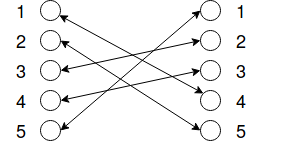
\includegraphics[scale=0.5]{premutation.png}
\end{figure}
\end{columns}
\end{frame}

\begin{frame}{Понятие назначения}
Мы можем
представлять назначение как некое биективное отображение $\phi$, которое ставит
элементы конечного множества $\mathrm{U}$ в соотвествие элементам конечного
множества $\mathrm{V}$.
\end{frame}

\begin{frame}{Связь перестановок и назначение}
назначение является перестановкой, которая записывается
в виде

\[
\left (
  \begin{tabular}{cccc}
  1 & 2 & \ldots & n\\
  $\varphi (1)$ & $\varphi (2)$ & \ldots & $\varphi (n)$
  \end{tabular}
\right )
\]
\end{frame}

\begin{frame}{Матрица назначений}
Каждой перестановке множества $\{1, 2, \ldots , n \}$ соответсвует единственная матрица
перестановок $\mathrm{X}_\varphi \in \mathrm{Matrix}_{n \times n}$, элементы котороый определяются как
\[
x_{ij} =
 \begin{cases}
   1 & \text{если } j = \varphi(i) \\
   0 & \text{иначе}
 \end{cases}
\]
Матрицу Х будем называть матрицей назначений
\end{frame}

\begin{frame}{Естественное обобщение ЗОН}
Рассмотрим обобщение ЗОН -- трехиндексную аксиальную задачу о назначениях

Она может быть определена следующим образом. 
Пусть даны $n^3$ весовых коэфициентов $c_{ijk}, (i,j,k=1 \ldots n)$. 
Необходимо найти такие перестановки $\varphi$ и $\xi$, что 
\[
  \min_{\varphi, \xi \in S_n} \sum^n_{i = 1} c_{i \varphi (i) \xi(i)}
\]

где $S_n$ множество всех перестановок целых чисел от $1 \ldots n$.
\end{frame}

\begin{frame}{3-АЗОН как ЗЛП}
Так же задача может быть переписана как задача целочисленного линейного программирования. 

\begin{eqnarray*}
  & \min \displaystyle \sum^n_{i = 1} \displaystyle \sum^n_{j = 1} \displaystyle \sum^n_{k = 1}
  c_{ijk} x_{ijk} \\
  \text{ограничения}
  &\displaystyle \sum^n_{i = 1} \displaystyle \sum^n_{k = 1} x_{ijk} = 1  &(j = 1, \ldots, n) \\
  &\displaystyle \sum^n_{j = 1} \displaystyle \sum^n_{k = 1} x_{ijk} = 1  &(i = 1, \ldots, n) \\
  &\displaystyle \sum^n_{i = 1} \displaystyle \sum^n_{j = 1} x_{ijk} = 1  &(k = 1, \ldots, n) \\
  & x_{ijk} \in \{ 0, 1 \} &(i,j,k = 1, \ldots, n)
\end{eqnarray*}
\end{frame}

\begin{frame}{Алгоритм, сводящий 3-АЗОН к двухмерному виду}
Пусть $\phi = X \rightarrow \mathbb{N}$ -- любая целочислено значащая функция, при этом $1 < \phi_n < n$ 
\begin{enumerate}
\item Берем произвольную подстановку $\pi \in S_n$. Пусть $(d_{jk})$ - $n \times n$ 
матрица, содержащая элементы исходной матрицы $(c_{ijk})$, где индекс $j=\pi(i)$ такой, что
$
d_{ij} = c_{\pi^{-1}(j)jk}
$
для любых $1 \leq j$,$n \leq n$
Положим $f = 0 ; j =1 ; \mathrm{K}={1,2, \ldots , \phi_n}$. 
\item Выберем номер $\sigma(j)$ минимального элемента из множества $\mathrm{argmin} \, {d_{jk} | k \in K}$.
\item Полагаем $f = f + d_{j \sigma (j)} ; \mathrm{K} = \mathrm{K}  \setminus  {\sigma(j)} ; k=j+\phi_n$
\item Если $k \leq n $, то $K = K \bigcap {k}$.
\item $j = j + 1$
\item Повторяем п.2, пока j<n. В противном случае идем к п.7
\item Результатом работы алгоритма $\mathrm{A}(\phi_n)$ является значение функции $f$ целевой функции   
$f_{\mathrm{A}(\phi_n)}$. 
\end{enumerate}
\end{frame}

\begin{frame}{Теоретическое обоснование}
Пусть весовые коэфициенты $c_{ijk} \in C$ лежат в отрезке $[a_n, b_n]$, $a_n>0$, $M_n$ -- множество всех возможных $C$. Тогда
\begin{block}{Теорема}
При $b_n / a_n = o(n/ \mathrm{ln} n)$ алгоритм является ассимптотически оптимальным для 3-АЗН на классе матриц $M_n$
и его временная сложность  $O(n^2)$.
\end{block}
\begin{block}{Теорема}
При $b_n / a_n = o(\mathrm{ln} n)$ алгоритм является ассимптотически оптимальным для 3-АЗН на классе матриц $M_n$
и его временная сложность  $O(n \mathrm{ln} n)$. 
\end{block}
\end{frame}

\begin{frame}{Выявленные недостатки. Предлагаемые модификации}
\begin{itemize}
\item Алгоритм чувствителен к выбору начальной перестановки
\item Показна сходимость алгоритма при $n \rightarrow \infty$, что неприменимо в практических задачах
\end{itemize}

Для исправления этих недостатков предлагаются следующие модификации к алгоритму
\end{frame}

\begin{frame}{Наивный итеративный алгоритм}
\Fontvi
\begin{enumerate}
\item положим счетчик $i=1$, зафикируем $p$ -- число итераций
\item Берем произвольную подстановку $\pi \in S_n$. Пусть $(d_{jk})$ - $n \times n$ 
матрица, содержащая элементы исходной матрицы $(c_{ijk})$, где индекс $j=\pi(i)$ такой, что
$
d_{ij} = c_{\pi^{-1}(j)jk}
$
для любых $1 \leq j$,$n \leq n$
Положим $f = 0 ; j =1 ; \mathrm{K}={1,2, \ldots , \phi_n}$. 
\item Выберем номер $\sigma(j)$ минимального элемента из множества $\mathrm{argmin} \, {d_{jk} | k \in K}$.
\item Полагаем $f = f + d_{j \sigma (j)} ; \mathrm{K} = \mathrm{K}  \setminus  {\sigma(j)} ; k=j+\phi_n$
\item Если $k \leq n $, то $K = K \bigcap {k}$.
\item $j = j + 1$
\item Повторяем п.3, пока j<n. В противном случае идем к п.7
\item Результатом работы итерации  $\mathrm{A_i}(\phi_n)$ на шаге $i$ является значение функции $f_i$ целевой функции   
$f_{\mathrm{A}(\phi_n)}$. 
\item i=i+1, если i<p, идем на п3
\item Результатом работы алгоритма $\mathrm{A}(\phi_n)$ является значение функции $f=\min_{i} {f_i}, \quad i=1 \ldots p$ 
\end{enumerate}
\end{frame}

\begin{frame}{Наивный итеративный алгоритм}
альтернативный вариант слайда

Итеративно запустим исходный алгоритм.
Получим множество решений $f = {f_i}$, $i = 1 \ldots p$, где $p$ -- количество итераций. 
Результатом работы алгоритма $\mathrm{A_2}(\phi_n)$ является $f=\min_{i} {f_i}, \quad i=1 \ldots p$ 
\end{frame}



\begin{frame}{Итеративный алгоритм с улучшением исходной перестановки} 
\Fontvi
\begin{enumerate}
\item положим счетчик $i=1$, зафикируем $p$ -- число итераций
\item Возьмем и запомним произвольную подстановку $\pi \in S_n$. 
\item Пусть $(d_{jk})$ - $n \times n$ 
матрица, содержащая элементы исходной матрицы $(c_{ijk})$, где индекс $j=\pi(i)$ такой, что
$d_{ij} = c_{\pi^{-1}(j)jk}$ для любых $1 \leq j$,$n \leq n$
Положим $f = 0 ; j =1 ; \mathrm{K}={1,2, \ldots , \phi_n}$. 
\item Выберем номер $\sigma(j)$ минимального элемента из множества $\mathrm{argmin} \, {d_{jk} | k \in K}$.
\item Полагаем $f = f + d_{j \sigma (j)} ; \mathrm{K} = \mathrm{K}  \setminus  {\sigma(j)} ; k=j+\phi_n$
\item Если $k \leq n $, то $K = K \bigcap {k}$.
\item $j = j + 1$
\item Повторяем п.3, пока j<n. В противном случае идем к п.7
\item Результатом работы итерации  $\mathrm{A_i}(\phi_n)$ является значение функции $f_i$ целевой функции   
$f_{\mathrm{A}(\phi_n)}$. 
\item Если $f_i < f_{i-1}$, случайным образом изменим 2 элемента $\pi$, иначе возьмем новую случайную  перестановку $pi$.
\item i=i+1, если i<p, идем на п3
\item Результатом работы алгоритма $\mathrm{A}(\phi_n)$ является значение функции $f$ целевой функции   
$f_{\mathrm{A}(\phi_n)}$. 
\end{enumerate}
\end{frame}

\begin{frame}{Наивный итеративный алгоритм}
альтернативный вариант слайда

Исходный алгоритм запускается итеративно. 
Вместо выбора новой случайной перестановки, введем перестановку $\pi'$, которая или получается из перестановки $\pi$ 
перестановкой двух случайных ее элементов, если текущий результат $f_i < f_{i-1}$, или является новой случайной перестановкой. 
Результатом работы алгоритма $\mathrm{A_3}(\phi_n)$ является значение функции $f$ целевой функции   
$f_{\mathrm{A_3}(\phi_n)}$. 

\end{frame}

\begin{frame}{Блок-схема алгоритма}
\begin{figure}
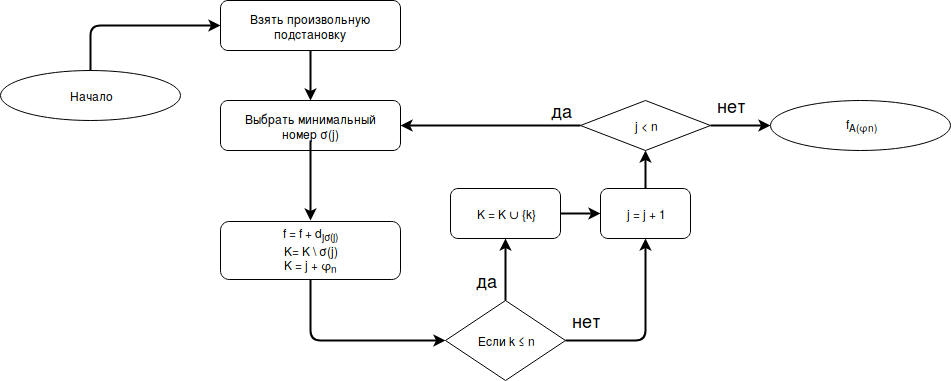
\includegraphics[scale=0.34]{algorithm.png}
\end{figure}
\end{frame}

\end{document}
